\chapter{El Framework FuD}
\label{fudcplusplus}

\epigraph{If you think it’s simple, then you
have misunderstood the problem.
}%
{\textbf{Bjarne Stroustrup}}

\section{El Framework FuD}
\par Computar grandes conjuntos de datos es una parte importante de las ciencias de la computación, mucha información es inherentemente complicada de comprimir y, además, los recursos para procesar estos conjuntos de datos son usualmente costosos. Las organizaciones sin fines de lucro, las instituciones educativas e instituciones similares deben encontrar otros caminos para administrar sus requerimientos de procesamientos mientras mantienen sus costos lo más bajo posible. Existen muchas herramientas para lograr una computación distribuida a bajo costo.

\par \textbf{FuD} (del acrónimo \emph{FuDePAN ubiquitous Distribution}) es un framework para la distribución de trabajos, o un framework para la implementación de aplicaciones distribuídas\cite{clus09}. Como tal, no depende del problema a implementar y no fuerza ningún modelo de comunicación o disposición de las unidades de procesamiento que serán utilizadas. 

\par \textbf{FuD} se organiza como un esquema \emph{Master-Worker} (un servidor y varios clientes conectados al mismo). Tanto cliente como servidor, se encuentran organizados en tres niveles separados (figura~\ref{disenioFud}), cada uno de ellos con una única responsabilidad bien definida. La comunicación entre los diferentes niveles se encuentra estrictamente
limitada, es decir, por cada nivel existe un único punto de comunicación ya sea para comunicarse con la capa
superior o con la inferior. Cuando un mensaje es creado, éste debe atravesar las diferentes capas comenzando
desde la de nivel más alto hacia la capa inferior, y luego recorrer en sentido contrario las capas del lado

\begin{figure}[h!] \hspace{.60cm}
    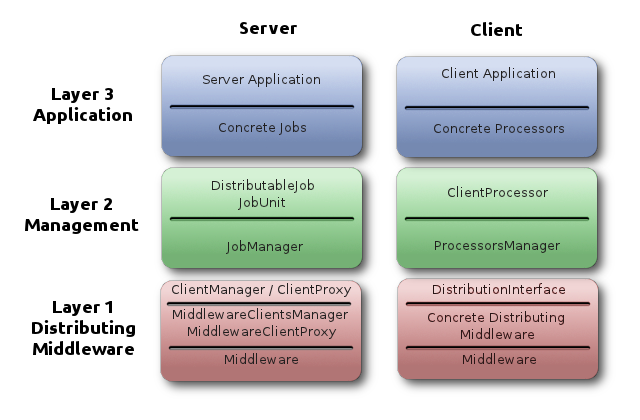
\includegraphics[scale=.55]{image/AbstractLayers.png}
    \caption{Vista abstracta de las capas de \textbf{FuD} [16].} 
    \label{disenioFud}
\end{figure}

\par \textbf{FuD} fue implementado empleando usando un esquema \emph{Divide \& Conquer} donde el procesamiento es llevado a cabo por los nodos procesadores. ``Divide'' cuando se realiza la división de un trabajo en una unidad de trabajo. ``Conquer'' al incorporar los resultados de una unidad de trabajo.

\subsection{Diseño}
A continuación se describe brevemente cada una de las capas que constituyen el framework.

\subsubsection{Application Layer (L3)} %aplicación
\par Básicamente proporciona los componentes que contienen todos los aspectos del dominio del problema a resolver. Estos aspectos incluyen todas las definiciones de los datos usados y su manipulación correspondiente, como así también todos los algoritmos relevantes para la solución al problema en general. 

\par Es necesario que del lado del servidor se implemente la aplicación principal, la cual hará uso de 	
una simple interfaz en la abstracción de un trabajo distribuible permitiendo así codificar la estrategia de
distribución de trabajos. Del lado cliente, solo se necesita implementar los métodos encargados de realizar
las computaciones indicadas por una unidad de trabajo.

\subsubsection{Job Management Layer (L2)} %manejador de trabajo
\par Esta capa permite manejar los trabajos que se desean distribuir como así también generar las unidades de
trabajo que serán entregadas a los clientes para su procesamiento. Estas unidades de trabajo llegan a su
cliente correspondiente gracias a la capa más baja, encargada de la distribución. Una vez finalizado el
procesamiento, se informa que todo ha terminado y otorga los resultados a la capa superior.

\subsubsection{Distributing Middleware Layer (L1)} %comunicación
\par En esta capa existe el único vínculo real entre clientes y servidor. La responsabilidad principal es manejar los clientes conectados al servidor y llevar a cabo los procedimientos de comunicación entre ambos.

\par Las implementaciones concretas de este nivel son variables y están determinadas por el middleware a
utilizar, por ejemplo \textsc{Boost.Asio}\footnote{\url{http://www.boost.org/doc/libs/1\_4\_00/doc/html/boost\_asio.html}}, \textsc{MPI}\footnote{\url{http://www.mcs.anl.gov/research/projects/mpi/}} o \textsc{BOINC}\footnote{\url{http://boinc.berkeley.edu/}}. 
		
\par Actualmente, \emph{FuD} cuenta con dos capas más, conocidas como \emph{FuD-RecAbs} y \emph{FuD-CombEng}. Estas capas no se describen dado que sólo se empleará \textbf{FuD} original, para mayor información \url{fud.googlecode.com.}

\subsection{Conceptos importantes}
Los siguientes conceptos son necesarios para entender el funcionamiento de una aplicación que usa FuD:
\begin{itemize}
	\item \emph{Cliente:} un cliente es una aplicación conectada al servidor y es el encargado de realizar las tareas de procesamiento.
	\item \emph{Trabajo:} un trabajo es cualquier tarea a realizar por la aplicación (también llamado trabajo distribuíble). Los mismos se
						  pueden subdividir en unidades de trabajo.
	\item \emph{Unidad de Trabajo:} representa un cómputo concreto y pertenece a un trabajo particular. No se puede dividir.
	\item \emph{Manejador de clientes:} módulo encargado de manejar los clientes conectados al servidor.
	\item \emph{Manejador de trabajos:} módulo de \textbf{FuD} encargado de llevar cuenta de los trabajos (de ambos tipos) que maneja el
										framework en un momento dado.
\end{itemize}
